% Chapter 6 --- Computational Architecture

\chapter{The Computational Architecture: From Pixel to Procurement Decision}\doublespacing
\label{Chapter6}
\lhead{Chapter V. \emph{Computational Architecture}}

%----------------------------------------------------------------------------------------
\section{Optoelectrical Parameter Optimisation}
%----------------------------------------------------------------------------------------

Auto White Balance (AWB) was identified as the primary source of chromatic instability in the imaging pipeline. AWB is designed for consumer photography, where the goal is perceptually natural colour rendering. In this application, that correction is counterproductive. The chromatic signals that AWB suppresses (subtle colour differences between \textit{Kernel Burnt} and dark-variety \textit{Pure Wheat}, early \textit{Black Tip} discolouration, and the surface sheen of \textit{Infested} grain) are the diagnostic cues the model depends on.

AWB was disabled and replaced with a fixed white-balance matrix calibrated under Drishti's specific illumination using a standard colour reference chart. Shutter speed was tuned to balance motion suppression during post-actuation grain settling against exposure level. WS2812B LED output was adjusted spatially to reduce specular reflections on glossy kernel surfaces \cite{LiWheat2024, ElMasry2019}. The result is a stable, repeatable optical signal: the same grain photographed across ten successive frames produces chromatically consistent images.

%----------------------------------------------------------------------------------------
\section{Dataset Acquisition and ML Model Training}
%----------------------------------------------------------------------------------------

% Note to author: Specific model architecture details, accuracy figures, and training
% hyperparameters should be completed once final training runs are concluded.

Public grain datasets do not represent the procurement network's specific wheat varieties, Drishti's illumination profile, or the partially dispersed sample states the device produces. Deploying a model trained on a generic dataset in a specific physical system introduces dataset shift, which tends to produce confident misclassification rather than uncertain prediction \cite{QuinoneroCandela2009}.

A domain-specific dataset was therefore built from scratch, capturing images through the same optical and mechanical pipeline described in Chapters~\ref{Chapter4} and~\ref{Chapter5}. Grain specimens were annotated across all twelve categories. Particular attention was given to the confusable pairs identified in fieldwork as most error-prone: \textit{Kernel Burnt} versus dark-variety \textit{Pure Wheat}, early \textit{Infested} versus \textit{Broken}, and \textit{Potia} versus immature \textit{Pure Wheat}.

Instance segmentation was selected over bounding-box detection. The $W/W\%$ calculation requires area estimation per category. Pixel-level masks produce more accurate area measurements than bounding boxes, which systematically overestimate the area of irregularly shaped grain bodies.

%----------------------------------------------------------------------------------------
\section{Edge-to-Server Software Architecture}
%----------------------------------------------------------------------------------------

\subsection{System Architecture Overview}

The Raspberry Pi 5 handles actuation control, GPIO timing, and image capture efficiently. It is not suited to running production-scale instance segmentation inference within the five-minute cycle target. A server-client architecture was adopted.

\begin{figure}[H]
    \centering
    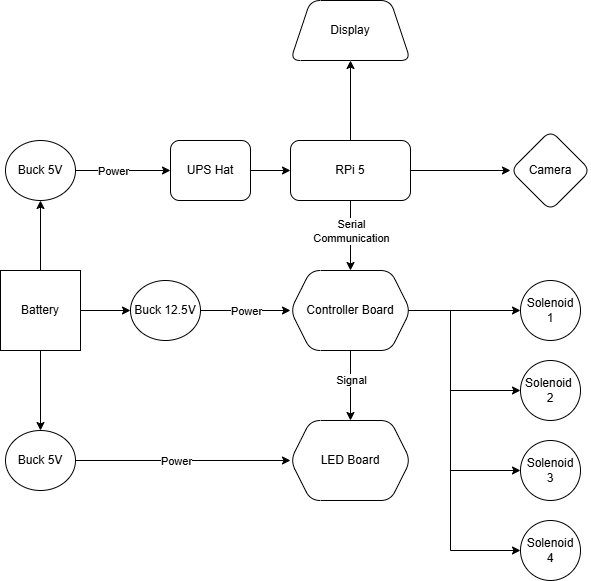
\includegraphics[width=0.9\textwidth]{Images/Drishti Hardware Architecture drawio.png}
    \caption{Drishti system architecture: the Raspberry Pi 5 edge node handles physical actuation and image capture; the central inference server handles segmentation and returns per-category $W/W\%$ results.}
    \label{fig:hardware_architecture}
\end{figure}

The Raspberry Pi 5 acts as the edge node: it manages actuation sequencing, captures images at calibrated parameters, applies lightweight preprocessing (resizing, calibration transforms, frame selection), and renders the local user interface. Preprocessed frames are transmitted over a local network to a central inference service. The service, exposed through a FastAPI endpoint, runs the instance segmentation model and returns per-category counts and $W/W\%$ values within the sub-five-minute window.

Running inference on a managed server allows model updates to be deployed centrally without physical access to field devices. Docker containerisation ensures consistent behaviour across the heterogeneous IT environments found at procurement sites \cite{Merkel2014}.
